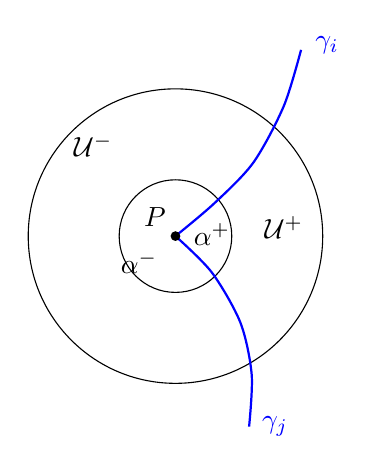
\begin{tikzpicture}[scale=1.1]
  \draw (0,0) circle (0.65);
  \draw (0,0) circle (1.7);
  % the two arcs meeting at P with a corner
  \draw[thick,blue] plot[smooth] coordinates {(0,0) (0.45,0.38) (0.9,0.85) (1.25,1.5) (1.45,2.15)};
  \draw[thick,blue] plot[smooth] coordinates {(0,0) (0.42,-0.42) (0.75,-1.0) (0.88,-1.6) (0.85,-2.2)};
  \node[blue] at (1.75,2.2) {$\gamma_i$};
  \node[blue] at (1.15,-2.2) {$\gamma_j$};
  \fill (0,0) circle (1.6pt) node[above left] {$P$};
  \node at (0.42,0.02) {$\alpha^+$};
  \node at (-0.42,-0.3) {$\alpha^-$};
  \node at (-0.95,1.05) {$\mathcal U^-$};
  \node at (1.25,0.1) {$\mathcal U^+$};
\end{tikzpicture}
